\documentclass{jarticle}

%%%%%%%%%%%%%%%%%%%%%%%%%%%%%%%%%%%%%%%%%%%%%%%%%%%%%%%%%%%%%%%%%%%%%%%%%%%
% packages
%%%%%%%%%%%%%%%%%%%%%%%%%%%%%%%%%%%%%%%%%%%%%%%%%%%%%%%%%%%%%%%%%%%%%%%%%%%
\usepackage{amsmath}
\usepackage{amssymb}
\usepackage{amsfonts}
\usepackage[dvipdfmx]{graphicx}
\usepackage[dvipdfmx]{color}
\usepackage{graphicx}
\usepackage{bm}
\usepackage[section]{placeins}
\usepackage{listings}

%%%%%%%%%%%%%%%%%%%%%%%%%%%%%%%%%%%%%%%%%%%%%%%%%%%%%%%%%%%%%%%%%%%%%%%%%%%
% format stuffs
%%%%%%%%%%%%%%%%%%%%%%%%%%%%%%%%%%%%%%%%%%%%%%%%%%%%%%%%%%%%%%%%%%%%%%%%%%%
\setlength{\oddsidemargin}{0.455cm} 
\setlength{\evensidemargin}{0.455cm} 
\setlength{\textwidth}{15.5cm} 
\setlength{\textheight}{22.54cm}
\setlength{\headheight}{0mm}
\setlength{\headsep}{0mm}
\setlength{\topskip}{0mm}
\setcounter{topnumber}{100}
\setcounter{bottomnumber}{100}
\setcounter{totalnumber}{100}
\renewcommand{\topfraction}{1.0}
\renewcommand{\bottomfraction}{1.0}
\renewcommand{\textfraction}{0.0}
\renewcommand{\floatpagefraction}{0.0}
\renewcommand{\baselinestretch}{1.0}
\pagestyle{empty}

%%%%%%%%%%%%%%%%%%%%%%%%%%%%%%%%%%%%%%%%%%%%%%%%%%%%%%%%%%%%%%%%%%%%%%%%%%%
% math symbols and commands
%%%%%%%%%%%%%%%%%%%%%%%%%%%%%%%%%%%%%%%%%%%%%%%%%%%%%%%%%%%%%%%%%%%%%%%%%%%
\newcommand{\eq}[1]{(\ref{#1})}
\newcommand{\mtx}[2]{\left[\begin{array}{#1} #2 \end{array}\right]}
\newcommand{\mycase}[1]{\left\{\begin{array}{ll} #1 \end{array} \right.}
\newcommand{\mb}[1]{\mbox{\boldmath$#1$}}
\newcommand{\lw}[1]{\smash{\lower2.ex\hbox{#1}}}
\newcommand{\zero}{\mathbf{0}}
\newcommand{\one}{\mathbf{1}}
\newcommand{\eps}{\varepsilon}

%%%%%%%%%%%%%%%%%%%%%%%%%%%%%%%%%%%%%%%%%%%%%%%%%%%%%%%%%%%%%%%%%%%%%%%%%%%
% colors
%%%%%%%%%%%%%%%%%%%%%%%%%%%%%%%%%%%%%%%%%%%%%%%%%%%%%%%%%%%%%%%%%%%%%%%%%%%
\newcommand{\myred}[1]{\textcolor{red}{#1}}
\newcommand{\myredbf}[1]{\textcolor{red}{\bf #1}}
\newcommand{\myblue}[1]{\textcolor{blue}{#1}}
\newcommand{\mybluebf}[1]{\textcolor{blue}{\bf #1}}
\newcommand{\mydarkblue}[1]{\textcolor[rgb]{0.0,0.0,0.5}{#1}}
\newcommand{\mygreen}[1]{\textcolor[rgb]{0.0,0.5,0.0}{#1}}
\newcommand{\mygreenbf}[1]{\textcolor[rgb]{0.0,0.5,0.0}{\bf #1}}
\newcommand{\mypurple}[1]{\textcolor[rgb]{0.5,0.0,0.5}{#1}}
\newcommand{\mypurplebf}[1]{\textcolor[rgb]{0.5,0.0,0.5}{\bf #1}}

\begin{document}
%%%%%%%%%%%%%%%%%%%%%%%%%%%%%%%%%%%%%%%%%%%%%%%%%%%%%%%%%%%%%%%%%%%%%%%%%%%
% ここからがレポートの記述
%%%%%%%%%%%%%%%%%%%%%%%%%%%%%%%%%%%%%%%%%%%%%%%%%%%%%%%%%%%%%%%%%%%%%%%%%%%

\begin{center} 
{\large \bf 知能プログラミング演習I 第4回レポート}
\end{center} %

\begin{flushright} 
\today \\% Date
\hskip 1mm
学籍番号 % 学籍番号
29114154\\
\hskip 1mm
氏名 % 氏名
PHAM DUY
\end{flushright} % Name

%%%%%%%%%%%%%%%%%%%%%%%%%%%%%%%%%%%%%%%%%%%%%%%%%%%%%%%%%%%%%%%%%%%%%%%%%%%
\section{レポートのテーマと構成}
\begin{itemize} 
\item テーマ\\
最近の深層学習について話題となっているgenerative adversarial network(GAN)の画像生成
\item 構成
\begin{itemize}
\item GANの内容
\item kerasを用いたGANの生成モデルの実装
\end{itemize}
\end{itemize}
%%%%%%%%%%%%%%%%%%%%%%%%%%%%%%%%%%%%%%%%%%%%%%%%%%%%%%%%%%%%%%%%%%%%%%%%%%%
\section{内容}
\subsection{概要}
GAN(Generative Adversarial Networks 日本語訳:「敵対的生成ネットワーク」)は生成モデルの一種であり、データから特徴を学習することで、実在しないデータを生成したり、存在するデータの特徴に沿って変換できる。GANは、正解データを与えることなく特徴を学習する「教師なし学習」の一手法として注目されている。そのアーキテクチャの柔軟性から、アイデア次第で広範な領域に摘用できる。応用研究や理論的研究も急速に進んでおり、今後の発展が大いに期待されている。
\begin{figure}
\centering
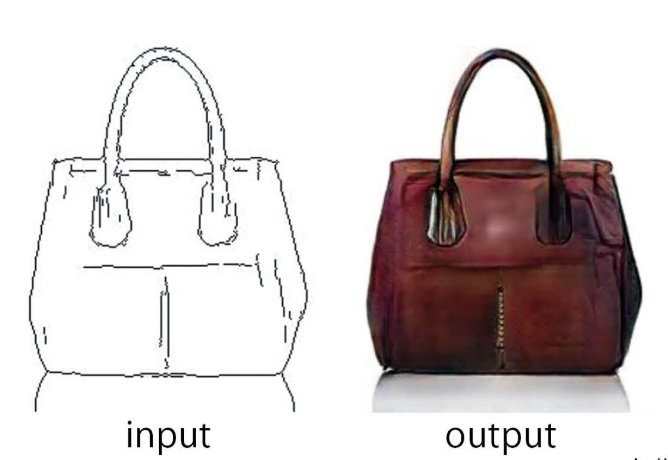
\includegraphics[width=10cm]{pic1.png}
\caption{GANによる画像生成}
\label{GANによる画像生成}
\end{figure}

\subsection{GANの発展の背景とその特徴}
\begin{itemize}
\item \textbf{発展の背景}\\
 GANは、イアン・グッドフェローらが2014年に発表した論文で、2つのネットワークを競わせながら学習させるアーキテクチャとして提案された。この斬新な構成により、従来の生成モデルより鮮明で本物らしい画像生成が可能になった。\\
 さらに2015年には、畳み込みニューラルネットワーク(CNN)で見られるような畳み込み層をネットワークに適用したDCGAN(Deep Convolutional GAN)が提案された。後述のように、GANは学習時に不安定になるケースが見られ、意味をなさない画像を生成したり、生成データの種類が偏るなどの課題があった。
\item \textbf{その特徴}\\
 GANは生成モデルであり、データの特徴を抽出して学習し、実在しないデータを生成できる。生成モデルに分類される手法としては、変分オートエンコーダやボルツマンマシンなども以前からあるが、GANはそれらの手法と比べてより鮮明な画像の生成が可能である。\\
\end{itemize}
\subsection{GANの学習の仕組み}
GANは、2つのニューラルネットワークで構成される。\\

GANは生成器と識別器がお互い、訓練中にナッシュ均衡を達成しようとする。GANのアーキテクチャを図1に示す。生成器Gの動作原理は実際のデータの潜在分布を極力適合させるために偽のデータを生成することである。一方で、識別器Dの動作原理は偽か実際のデータか正しく見分けることである。生成器の入力はランダムノイズベクトルz(基本的には一様分布もしくは正規分布)である。ノイズは多次元ベクトルである偽のサンプルG(z)を得るために生成器Gを介して新しいデータ空間にマッピングされる。また、識別器Dは二値分類器でありデータセットからの実際のサンプルもしくは生成器Gから生成された偽のサンプルを入力として受け取る。そして、識別器Dの出力は実際のデータである確率である。識別器Dが実際のものか偽のものかどうかわからなくなった時、GANは最適な状態になる。この時点で、実際のデータ分布を学習した生成器モデルGが得られる。
\begin{figure}[h]
\centering
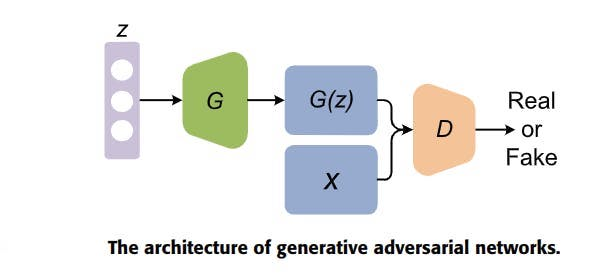
\includegraphics[width=14cm]{pic3.jpeg}
\caption{GANのアーキテクチャ}
\label{GANのアーキテクチャ}
\end{figure}

\subsection{GANの学習モデル}
$J\textsuperscript{(G)}$と$J\textsuperscript{(D)}$をそれぞれ識別器損失関数と生成器の損失関数とする。識別器$D$が二値分類器として定義され、損失関数はクロスエントロピーで示される。定義は式(1)の通り。\\
\begin{equation}
\centering
J^{(G)}=-\frac{1}{2}\mathbb{E}_{x\sim pdata}logD(x)-\frac{1}{2}\mathbb{E}_zlog(1-D(G(z)))
\end{equation}

ここで、$x$は実際のサンプルを示し、$z$は$G(z)$を生成器$G$で生成するためのランダムノイズベクトル、$\mathbb{E}$は期待(期待値、expectation)である。$D(x)$は$D$が$x$を実際のデータとみなす確率、$D(G(z))$は$D$が$G$によって生成されたデータを特定する確率を示す。$D$の目的はデータの出所を正しく突き止めることであるため、$D(G(z))$が0に近づくことを目標とするが、$G$は1に近づくことを目的とする。この考えに基づいて、2つのモデル間には対立が存在する(ゼロサムゲーム)。したがって、生成器の損失は識別機によって式(2)の様に導出される。\\
\begin{equation}
\centering
J^{(G)}=-J^{(D)}
\end{equation}
結果的に、GANの最適化問題はminimaxゲームに変換される。定義は式(3)の通り。\\
\begin{equation}
\centering
\min_{G} max_{D} (D,G) = \mathbb{E}_{x\sim pdata(x)}[logD(x)]+\mathbb{E}_{z\sim p(z)}[log(1-D(G(z)))]
\end{equation}
訓練プロセス中に$G$中のパラメーターは$D$の更新プロセスのパラメーターと一緒に更新される。$D(G(z))=0.5D(G(z))=0.5$である時、識別機はこれらの2つの分布間の差異を特定することができなくなる。この状態では、モデルが大域的最適解を達成するだろう。

\subsection{派生GANモデル}
オリジナルのGANsの欠陥により、様々な派生GANsモデルが提案され、これらの派生GANsモデルはアーキテクチャ最適化ベースのGANsと目的関数最適化ベースのGANsの2種類のグループに分けられる(図3)。このセクションでは、いくつかの派生モデルの詳細について紹介する。\\
\begin{figure}[h]
\centering
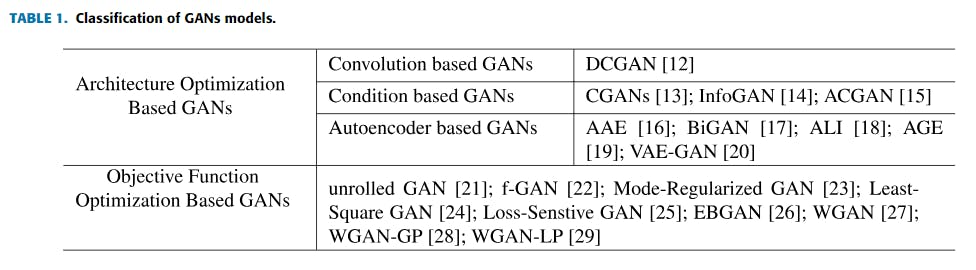
\includegraphics[width=14cm]{pic4.jpeg}
\caption{派生GANモデル}
\label{GAN3}
\end{figure}

\textbf{GANの応用研究}

\begin{itemize}
\item \textbf{Conditional GAN(条件付きベースのGAN)}\\
通常のGANのデータ生成は、ランダムにサンプルされるので、生成されるデータの種類を制御できない。Conditional GANは学習時にラベルを与えることで、推論時にもラベルを入力してデータを生成できる。図4はその例で、数字の種類を指定してデータを生成している。
\begin{figure}[h]
\centering
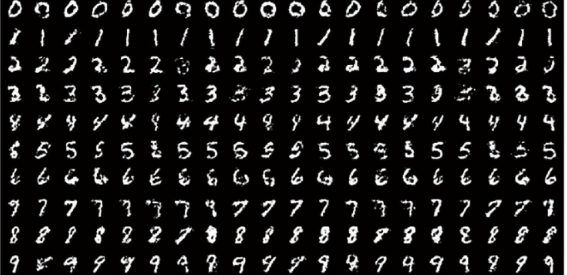
\includegraphics[width=12cm]{pic5.png}
\caption{条件付きベースのGANによるデータ生成(MNISTデータセット)}
\label{GAN4}
\end{figure}

\item \textbf{SRGAN}\\
低解像度の画像を高解像度に復元する、超解像を目的としたGANである。Bicubic法のような従来の超解像手法による復元では、ぼやけた画像になりやすい。SRGANでは、GANの特性を利用することで、ぼやけの少ない画像の復元が可能である。
\item \textbf{pix2pix}\\
 pix2pixは画像間の特徴を変換する。図5では、セグメンテーションされた景色に対して、たとえば「航空写真を地図化する」「日中の写真を夜間のシーンに変換する」などを行っており、入力時に変換前の画像をラベルとして与えるconditional な設定と考えられる。「ある特徴をもつ画像から、別の特徴へ変換する」と捉えると、応用アイデアが広がる。
\begin{figure}[h]
\centering
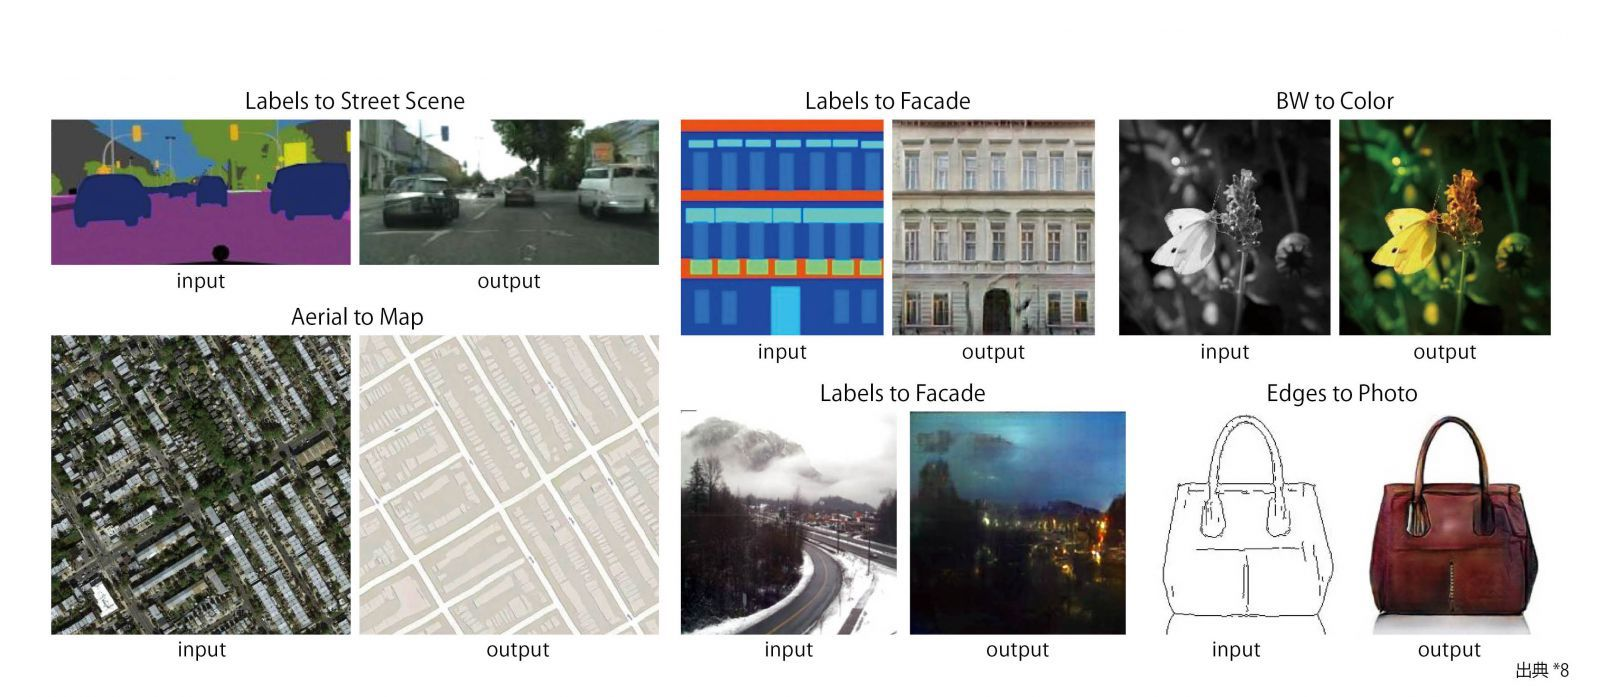
\includegraphics[width=12cm]{pic6.jpg}
\caption{pix2pixにより画像間の特徴を変換する}
\label{GAN5}
\end{figure}

\item \textbf{Cycle GAN}\\
pix2pixと同じく、画像の特徴間の変換を実行する。ウマとシマウマを変換した図6がこの手法を使用している。ここでは学習データの変換元と変換先の対応付けが必要なく、共通した特徴(ドメインと呼ぶ)をもつ画像を集めて、GeneratorとDiscriminatorのそれぞれに学習させることで、各特徴間を相互に変換する。
\begin{figure}[h]
\centering
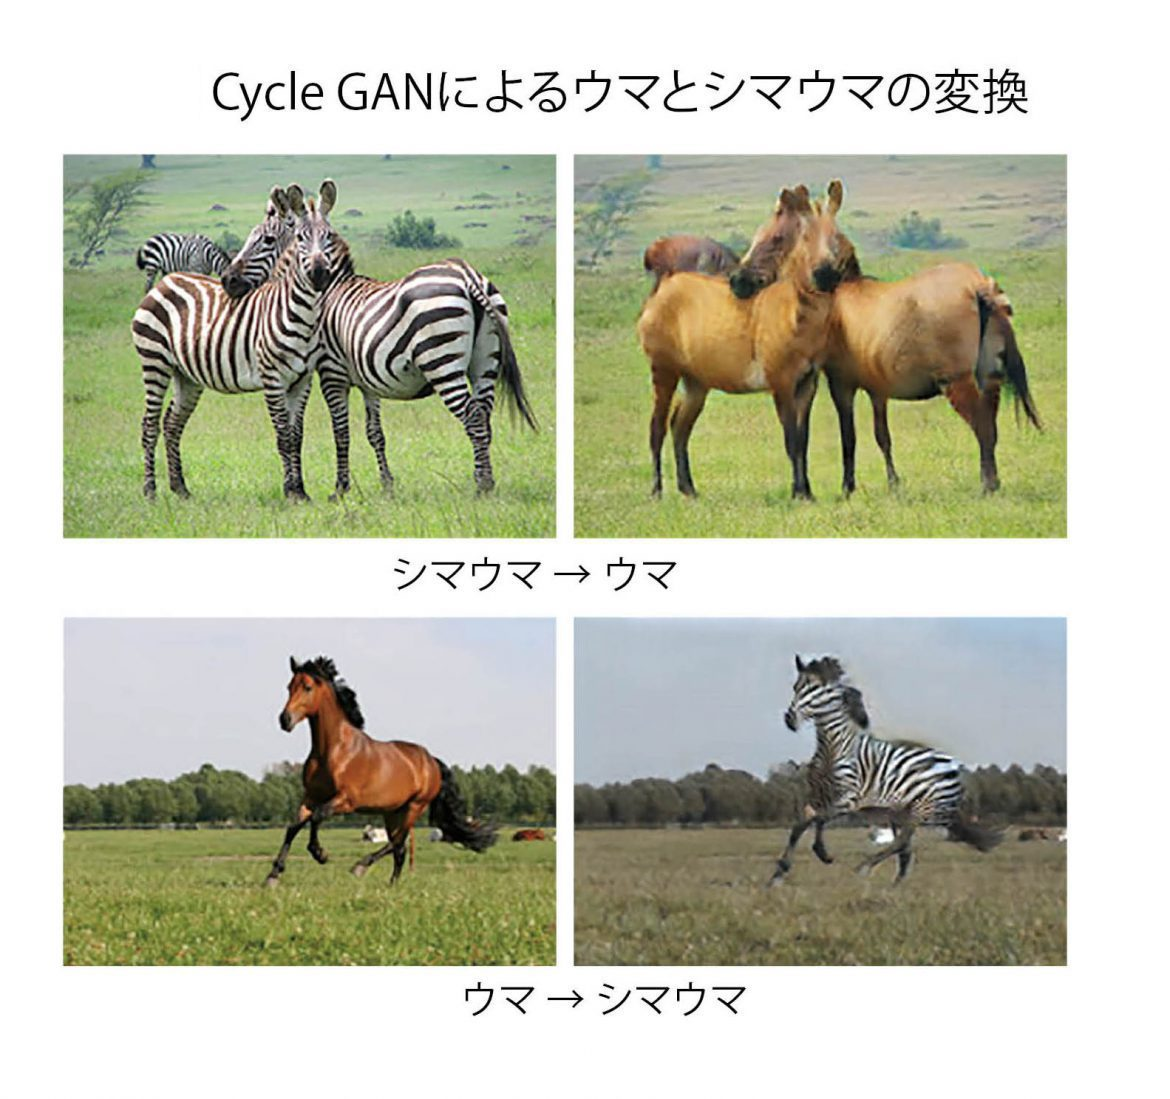
\includegraphics[width=12cm]{pic7.jpg}
\caption{Cycle GANによる馬とシマウマの変換}
\label{GAN6}
\end{figure}

\end{itemize}

%%%%%%%%%%%%%%%%%%%%%%%%%%%%%%%%%%%%%%%%%%%%%%%%%%%%%%%%%%%%%%%%%%%%%%%%%%%
%%%%%%%%%%%%%%%%%%%%%%%%%%%%%%%%%%%%%%%%%%%%%%%%%%%%%%%%%%%%%%%%%%%%%%%%%%%
\section{kerasを用いたGANの生成モデルの実装}
今回ConditionalGANをKerasで実装する。
\textbf{ソースコード}
\lstinputlisting[language=Python]{conditionalGAN.py}

\textbf{出力結果}
\begin{figure}[h]
\centering
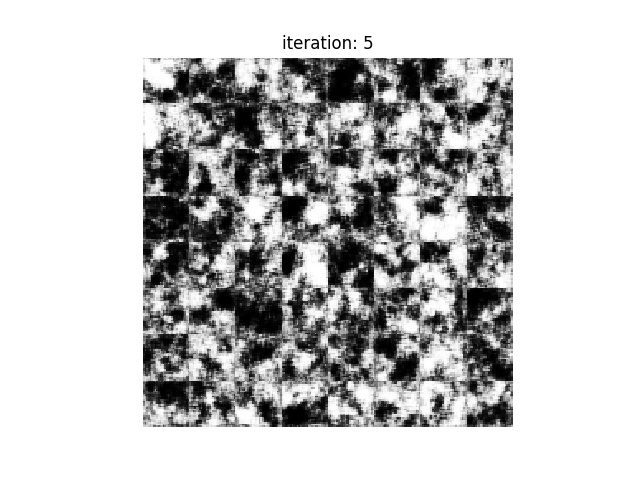
\includegraphics[width=12cm]{0005.jpg}
\caption{ConditionalGANによる画像生成の例(MNIST DATASETより)}
\label{GAN7}
\end{figure}


%%%%%%%%%%%%%%%%%%%%%%%%%%%%%%%%%%%%%%%%%%%%%%%%%%%%%%%%%%%%%%%%%%%%%%%%%%%
% ここまでがレポートの記述
%%%%%%%%%%%%%%%%%%%%%%%%%%%%%%%%%%%%%%%%%%%%%%%%%%%%%%%%%%%%%%%%%%%%%%%%%%%
\end{document}
